\documentclass{article}
\usepackage{pgfplots}
\usepackage{pgfplotstable}

\pgfplotsset{compat=1.18}

\begin{document}

\begin{figure}
    \centering
    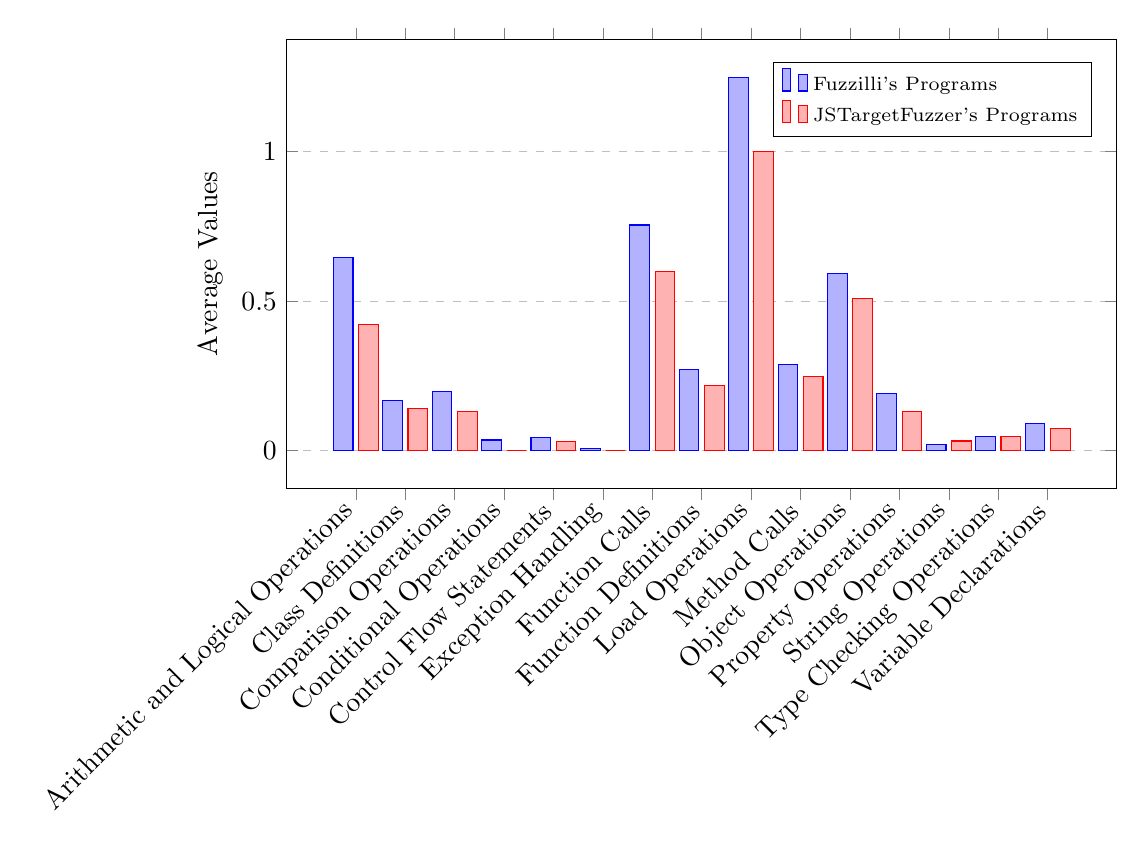
\begin{tikzpicture}
        \begin{axis}[
            ybar,
            bar width=.25cm,
            width=\textwidth,
            height=.6\textwidth,
            symbolic x coords={
                Arithmetic and Logical Operations, 
                Class Definitions, 
                Comparison Operations,
                Conditional Operations,
                Control Flow Statements,
                Exception Handling,
                Function Calls,
                Function Definitions,
                Load Operations,
                Method Calls,
                Object Operations,
                Property Operations,
                String Operations,
                Type Checking Operations,
                Variable Declarations
            },
            xtick=data,
            x tick label style={rotate=45, anchor=east},
            enlarge x limits=0.1,
            ylabel={Average Values},
            legend style={at={(0.97,0.95)}, anchor=north east},
            ymajorgrids=true,
            grid style=dashed,
            ylabel style={align=center},
            legend cell align={left},
            legend style={font=\scriptsize}
        ]
        \addplot coordinates {(Arithmetic and Logical Operations,0.644338) (Class Definitions,0.168613) (Comparison Operations,0.197040) (Conditional Operations,0.036019) (Control Flow Statements,0.044653) (Exception Handling,0.006302) (Function Calls,0.754542) (Function Definitions,0.271438) (Load Operations,1.248671) (Method Calls,0.288207) (Object Operations,0.591108) (Property Operations,0.191801) (String Operations,0.020139) (Type Checking Operations,0.046969) (Variable Declarations,0.090158)};
        \addplot coordinates {(Arithmetic and Logical Operations,0.420732) (Class Definitions,0.140429) (Comparison Operations,0.130081) (Conditional Operations,0.000000) (Control Flow Statements,0.031098) (Exception Handling,0.000000) (Function Calls,0.597561) (Function Definitions,0.217636) (Load Operations,1.000000) (Method Calls,0.247967) (Object Operations,0.507317) (Property Operations,0.131243) (String Operations,0.032520) (Type Checking Operations,0.048780) (Variable Declarations,0.073171)};
        \legend{Fuzzilli's Programs, JSTargetFuzzer's Programs}
        \end{axis}
    \end{tikzpicture}
    \caption{Average Values by Category}
\end{figure}

\end{document}
